\documentclass[12pt, a4paper, twoside]{article}
\usepackage[utf8]{inputenc}
\usepackage[cm]{fullpage}
\usepackage{fancyhdr}
\usepackage{textcomp}
\usepackage{graphicx}

\begin{document}

\title{Relatório do Experimento 3 de OAC}
\author{
Arthur Bizzi: 13/0102636 \\
Arthur da Silveira Couto: 16/0002575 \\
Caio Albuquerque Brandão: 16/0003636 \\
Cristiano Silva Júnior: 13/0070629 \\
Leonardo Maffei: 16/0033811 \\}
\date{7 de Junho de 2017}
\maketitle

\section{Exercício 1}

\subsection{Parte A}

\subsection{Exercício 4}

O código no arquivo \textit{SYSTEMv53.s} descreve uma rotina de tratamento de exceções, como evidenciado na figura 1.

% Como adicionar uma figura
\begin{figure}
    \centering
    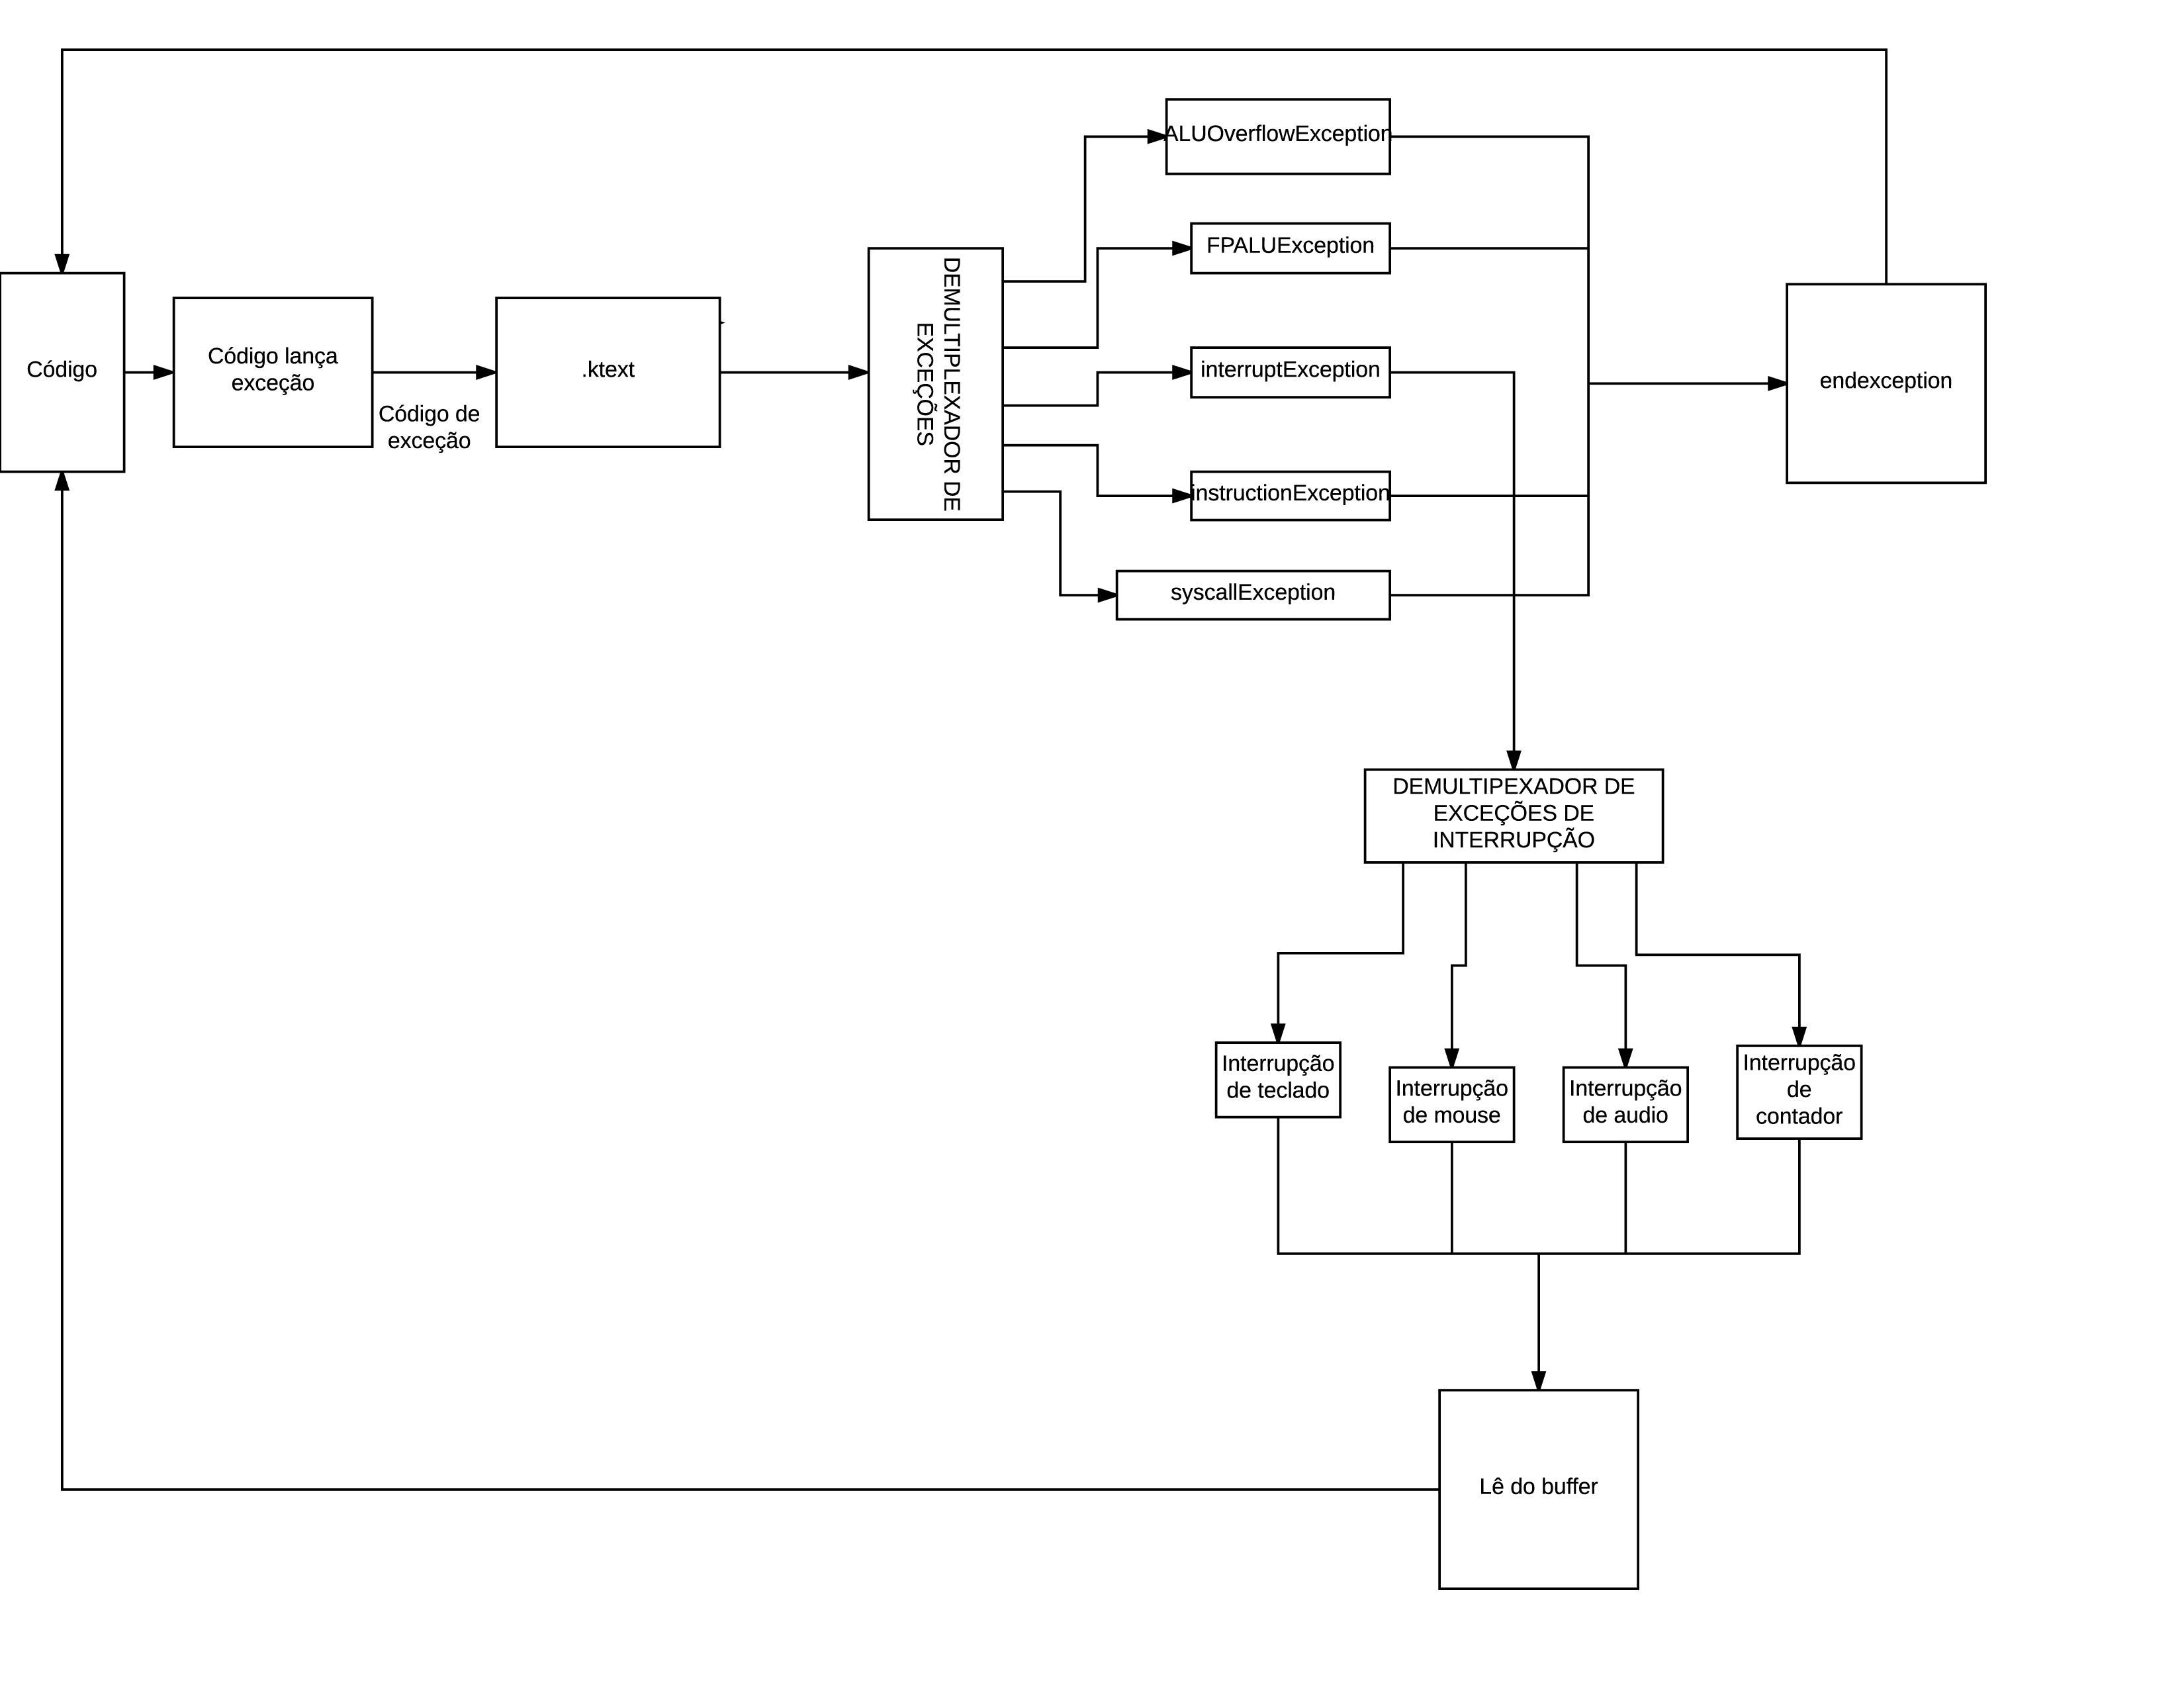
\includegraphics[width=0.8\textwidth]{./figs/f1-4.png}
    \caption{Diagrama do fluxo de tratamento de exceções}
\end{figure}

\section{Parte B}

\subsection{Exercício 7}

Analisando o código em \textit{Verilog} do processador descrito no projeto \textit{MIPS-PUM-v4.8}, podemos construir o diagrama de blocos presente na figura 2 para descrever a estrutura do processador a nível de estruturas funcionais.

\begin{figure}
    \centering
    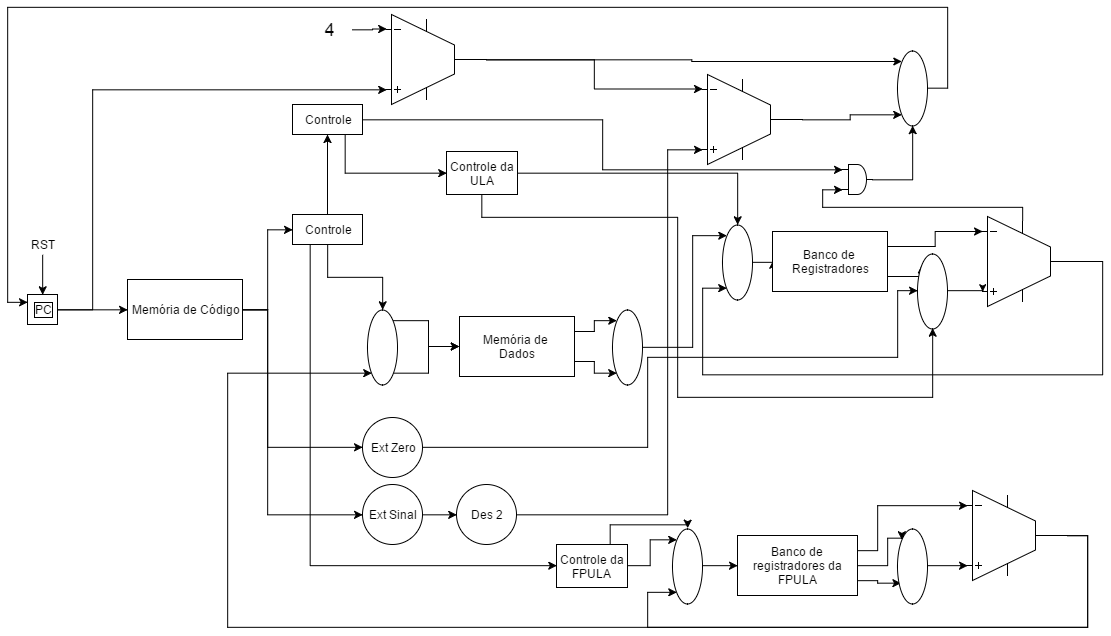
\includegraphics[width=0.8\textwidth]{./figs/UNICICLO.png}
    \caption{Diagrama de blocos do processador uniciclo}
\end{figure}

\subsection{Exercício 8}

O arquivo \textit{teste.s} contém uma rotina de testes para as instruções implementadas em sala de aula. Ela consiste basicamente em testar se uma operação funciona com um conjunto de dados conhecidos. Caso ela falhe, o programa cai em uma subrotina \textit{FU}, que termina o programa abruptamente.

\subsection{Exercício 9}

Para sintetizar a FPULA no processador em questão, basta descomentar a linha \textit{\` define FPU} e reorganizar as conexões e dispositivos que conversam com esta ULA, para que eles sejam definidos somente com esta diretiva. Desta forma, foi possível comparar o sintetizador com e sem a FPULA. A diferença entre os requisitos físicos está descrito na tabela 1.

\begin{center}
  \begin{tabular}{ | c | c | c | }
    \hline
    Parâmetro                  & Sem FPULA & Com FPULA \\ \hline \hline
    \# de elementos lógicos    & 15922     & 24497     \\ \hline
    \# de registradores        & 3431      & 6742      \\ \hline
  \end{tabular}
\end{center}

O número de registradores dobra pois a FPULA demanda praticamente outro processador (o chamado coprocessador 1) para poder realizar seus cálculos.

\subsection{Exercício 10}

Para se implementar as funções \textit{ceil}, \textit{floor} e \textit{round} no processador em questão, nao se deve fazer mudanças no caminho de dados, já que todas as unidades operacionais contidas no processador são capazes de realizar as instruções em questão. Contudo, a lógica de controle da FPULA deve ser atualizada para levar em consideração mais 3 novas instruções, cada uma com seu \textit{OPCODE} e seu \textit{FUNCT} definidos.



\end{document}
